\chapter{Template}
\label{sec:template}

\section{Instructions}

\begin{description}
\item[\textcolor{green}{Author}] Author of the approaches description  \todo{Name -  Company}
\item[\textcolor{blue}{Assessor 1}] First assessor of the approaches \todo{Name - Company}
\item[\textcolor{magenta}{Assessor 2}] Second assessor of the approaches \todo{Name - Company}
\end{description}

In the sequel, main text is under the responsibilities of the author.

\begin{author_comment}
Author can add comments using this format at any place.
\end{author_comment}

\begin{assessor1}
First assessor can add comments using this format at any place.
\end{assessor1}

\begin{assessor2}
Second assessor can add comments using this format at any place.
\end{assessor2}

When a note is required, please follow this list :
\begin{description}
\item[0] not recommended, not adapted, rejected
\item[1] weakly recommended, adapted after major improvements, weakly rejected
\item[2] recommended, adapted (with light improvements if necessary)  weakly accepted
\item[3] highly recommended, well adapted,strongly accepted
\item[*] difficult to evaluate with a note (please add a comment under the table)
\end{description}

All the notes can be commented under each table.

\section{Presentation}

This section gives a quick presentation of the approach and the tool.

\begin{description}
\item[Name] \todo{Name of the approach and the tool}
\item[Web site] \todo{if available, how to  find information}
\item[Licence] \todo{Kind of licence}
\end{description}

\paragraph{Abstract} Short abstract on the approach and tool (10 lines max)

\paragraph{Publications} Short list of publications on the approach (5 max)


For which activities are dedicaded the means or tools (give a note from 0 to  3) :

\begin{tabular}{|l | c | c | c | c|}
\hline
& \textcolor{green}{Author} & \textcolor{blue}{Assessor 1} & \textcolor{magenta}{Assessor 2} & Total \\
\hline 
Verification (WP4) & & & &  \\
\hline
Validation (WP4) & & & & \\
\hline
Safety analysis (WP4) & & & & \\
\hline
Data, function or requirement management & & & & \\
(SSRS, WP3 and WP4) & & & & \\
\hline
Model or code transformation (WP3 and WP4) & & & & \\
\hline
\end{tabular}

According the results of this table, some of the following sections can be skipped.

\section{Common criteria on secondary means and tools}
\label{common}
This section discusses the common criteria of the means and tools according to the project requirements on tools and the results of T7.1.

\subsection{Project and WP2 requirements}

The objectives of this list of criteria is to check if the proposed means and tools meet the main criteria of the project: open-source approaches, usability, modularity, coverage of the objectives,...

According WP2 requirements, give a note for characteristics of the use of the tool (from 0 to 3) :

\begin{tabular}{|l | c | c | c | c|}
\hline
& \textcolor{green}{Author} & \textcolor{blue}{Assessor 1} & \textcolor{magenta}{Assessor 2} & Total \\
\hline 
Open Source (D2.6-02-074) & & & &  \\
\hline 
Portability to operating systems (D2.6-02-075) & & & &  \\
\hline
Cooperation of tools (D2.6-02-076) & & & &  \\
\hline
Robustness (D2.6-02-078) & & & & \\
\hline
Modularity (D2.6-02-078.1) & & & & \\
\hline
Documentation management (D2.6-02-078.02) & & & & \\
\hline
Distributed software development (D2.6-02-078.03)  & & & & \\
\hline
Simultaneous multi-users (D2.6-02-078.04)   & & & & \\
\hline
Issue tracking (D2.6-02-078.05) & & & & \\
\hline
Differences between models (D2.6-02-078.06) & & & & \\
\hline
Version management (D2.6-02-078.07) & & & & \\
\hline
Concurrent version development (D2.6-02-078.08) & & & & \\
\hline
Model-based version control (D2.6-02-078.09) & & & & \\
\hline
Role traceability (D2.6-02-078.10) & & & & \\
\hline
Safety version traceability (D2.6-02-078.11) & & & & \\
\hline
Model traceability (D2.6-02-079) & & & & \\
\hline
Tool chain integration & & & & \\
\hline
Scalability & & & & \\
\hline
\end{tabular}



\subsection{Qualification}

This section discusses how the tool can be classified according EN50128 requirements (D2.6-02-085). Some qualification shall be mandatory  if the tool is involved to design a SIL4 software.


\begin{tabular}{|l | c | c | c | c|}
\hline
& \textcolor{green}{Author} & \textcolor{blue}{Assessor 1} & \textcolor{magenta}{Assessor 2} & Total \\
\hline 
Tool manual (D.2.6-01-42.02) & & & &  \\
\hline
Proof of correctness (D.2.6-01-42.03)   & & & & \\
\hline
Existing industrial  usage  & & & & \\
\hline
Model verification & & & & \\
\hline
Test generation & & & & \\
\hline
Simulation, execution, debugging & & & & \\
\hline
Formal proof & & & & \\
\hline
\end{tabular}


Which scope of qualification is expected according EN50128 (section 6.7) ?

\begin{tabular}{|l | c | c | c | c|}
\hline
& \textcolor{green}{Author} & \textcolor{blue}{Assessor 1} & \textcolor{magenta}{Assessor 2} & Total \\
\hline 
class T1 & & & &  \\
\hline
class T2   & & & & \\
\hline
class T3  & & & & \\
\hline
\end{tabular}

\paragraph{Other elements for tool certification}


\subsection{Complementarity with primary toolchain}

The objectives of this list of criteria is to check if the proposed means and tools can be easily integrated to the primary toolchain.


According to the decisions and the propositions of T7.1, how the mean and approach can be adapted to or can complete:

\begin{tabular}{|l | c | c | c | c|}
\hline
& \textcolor{green}{Author} & \textcolor{blue}{Assessor 1} & \textcolor{magenta}{Assessor 2} & Total \\
\hline 
Eclipse & & & &  \\
\hline
SysML  & & & & \\
\hline
Papyrus  & & & & \\
\hline
Scade & & & & \\
\hline
EFS & & & & \\
\hline
Classical B approach & & & & \\
\hline
C code & & & & \\
\hline
\end{tabular}

\paragraph{Eclipse}
How the means or tools can be adapted to the Eclipse platform ?

\paragraph{SysML and Papyrus}
How the means or tools can complete SysML with Papyrus ?


\paragraph{Scade, EFS, Classical B}
How the means or tools can complete the current proposals for formal modeling ?

\paragraph{C code}
How the means or tools can complete or be adapted to SIL4 software in C code ?



\section{Means and tools for verification and validation purposes}
\label{sec:vnv}

This section defines the criteria for the means and tools dedicated to verification and validation activities, in the WP4 workpackage. 

Criteria of this section are defined according \citep{D4.1}.

\subsection{VnV Activities}

The VnV activities are described in details in the verification and Validation Plan  \citep{D4.1}.

\begin{figure}[htb]
  \centering
  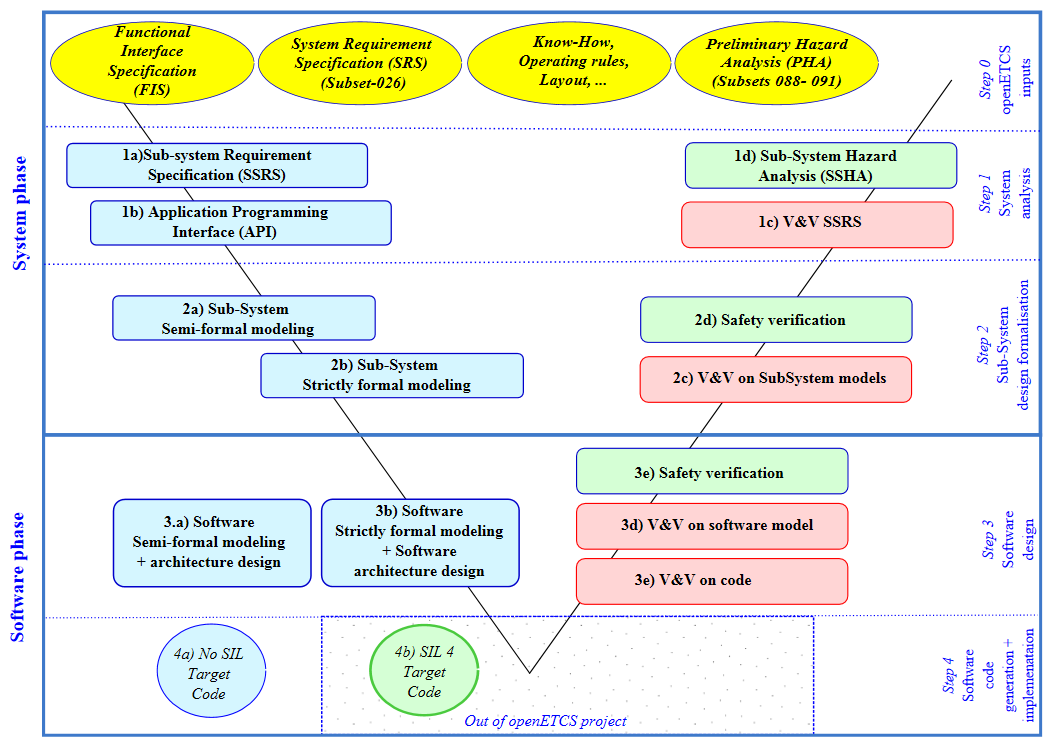
\includegraphics[width=.9\textwidth]{images/ProcessOpenETCS-BeM.png}
  \caption{openETCS Process (rough view)}
  \label{fig:openETCSProcess}
\end{figure}

According figure \ref{fig:openETCSProcess}, for which activities is the mean or tool suitable (see also \citep{D4.1} section 5.1.2 for more details) ?


\begin{tabular}{|l | c | c | c | c|}
\hline
& \textcolor{green}{Author} & \textcolor{blue}{Assessor 1} & \textcolor{magenta}{Assessor 2} & Total \\
\hline 
1c SSRS Verification & & & &  \\
\hline
1c SSRS Validation & & & &  \\
\hline
2c SFM Verification & & & &  \\
\hline
2c SFM Validation & & & &  \\
\hline
3d SW-SFM Verification & & & &  \\
\hline
3d SW-SFM Validation & & & &  \\
\hline
3d SW-FFM Verification & & & &  \\
\hline
3d SW-FFM Validation & & & &  \\
\hline
3e Code Verification & & & &  \\
\hline
3e Code Validation & & & &  \\
\hline
\end{tabular}


\subsection{Properties}

Which kind of properties or elements are verified or validated by the mean or tool (see also \citep{D4.1} section 4)  ?



\begin{tabular}{|l | c | c | c | c|}
\hline
& \textcolor{green}{Author} & \textcolor{blue}{Assessor 1} & \textcolor{magenta}{Assessor 2} & Total \\
\hline 
Functionalities of the system and sub-system & & & &  \\
\hline
System and sub-system architecture & & & &  \\
\hline
External and internal interfaces of sub-system & & & &  \\
\hline
Software components & & & &  \\
\hline
Performance constraints & & & &  \\
\hline
Safety objectives & & & &  \\
\hline
Functional properties & & & &  \\
\hline
Safety properties & & & &  \\
\hline
\end{tabular}



\subsection{Verification methods and tools}

Which kind of methods is proposed (see also \citep{D4.1} section 5.3) ?



\begin{tabular}{|l | c | c | c | c|}
\hline
& \textcolor{green}{Author} & \textcolor{blue}{Assessor 1} & \textcolor{magenta}{Assessor 2} & Total \\
\hline 
Reviews & & & &  \\
\hline
Inspections & & & &  \\
\hline
Software Architecture Analysis Method & & & &  \\
\hline
Architecture Tradeoff Analysis Method & & & &  \\
\hline
Model-Based System Integration Testing & & & &  \\
\hline
Model-Based Testing of Generated High-Level Code & & & &  \\
\hline
Abstract Interpretation & & & &  \\
\hline
Deductive Verification & & & &  \\
\hline
Model Checking & & & &  \\
\hline
Correct by Construction Formal Methods & & & &  \\
\hline
Verification with Formal Methods & & & &  \\
\hline
Simulation-based & & & &  \\
\hline
\end{tabular}

\subsection{Validation means and tools}

The following list of criteria focuss on means and tools to support validation activities, according WP2  requirements :

\begin{tabular}{|l | c | c | c | c|}
\hline
& \textcolor{green}{Author} & \textcolor{blue}{Assessor 1} & \textcolor{magenta}{Assessor 2} & Total \\
\hline 
Simulation-based & & & &  \\
\hline
Step-by-step simulation (D2.6-01-036) & & & &  \\
\hline
Environment emulation (D2.6-01-037 and D2.6-02-080) & & & &  \\
\hline
Time-based test case (D2.6-02-081) & & & &  \\
\hline
Test cases writing (D2.6-01-038) & & & &  \\
\hline
Test cases execution (D2.6-01-038) & & & &  \\
\hline
Test cases storage (D2.6-01-038) & & & &  \\
\hline
Version management of test cases (D2.6-02-082) & & & &  \\
\hline
Test generation from independant test model (D2.6-02-083) & & & &  \\
\hline
Test sequences writing (D2.6-02-084) & & & &  \\
\hline
Test sequences execution (D2.6-02-084) & & & &  \\
\hline
Test sequences storage (D2.6-02-084) & & & &  \\
\hline
\end{tabular}

\subsection{Other Criterias}



\begin{comment}
MPD : Todo
Ideas welcomed !

\end{comment}





\section{Means and tools for safety activities support}
\label{sec:safety}


This section defines the criteria for the means and tools dedicated to support of safety activities, in the WP4 workpackage. 

Criteria of this section are defined according \citep{D4.2.a}.

\subsection{Safety activities}

Which safety design activities are covered by the mean or tool (see \citep{D4.2.a} section 1.2) ?

\begin{tabular}{|l | c | c | c | c|}
\hline
& \textcolor{green}{Author} & \textcolor{blue}{Assessor 1} & \textcolor{magenta}{Assessor 2} & Total \\
\hline 
Preliminary Hazard Analysis & & & &  \\
\hline
Establish Safety Plan & & & & \\
\hline
System Hazard and Risk Analysis & & & & \\
\hline
Risk Assessment & & & & \\
\hline
Specification of System Safety Requirements & & & &  \\
\hline
Define Safety Related Functional Requirements & & & & \\
\hline
Specify Sub-System and Component & & & & \\
Safety requirements & & & & \\
\hline
Implement Safety Plan & & & & \\
\hline
Verify System, Sub-System and Component & & & &  \\
Safety requirements & & & &  \\
\hline
Validate System Safety Requirements & & & & \\
\hline
Establish Safety Case & & & & \\
\hline
\end{tabular}


\subsection{Input Artifacts}

Which artifacts are used as input of the mean or tool (see \citep{D4.2.a} section 1.4) ? 


\begin{tabular}{|l | c | c | c | c|}
\hline
& \textcolor{green}{Author} & \textcolor{blue}{Assessor 1} & \textcolor{magenta}{Assessor 2} & Total \\
\hline 
Safety Requirement & & & &  \\
\hline
Hazard log & & & & \\
\hline
Safety Plan & & & & \\
\hline
Safety Case & & & & \\
\hline
Code Safety Backlog & & & &  \\
\hline
Detailed Model Safety Backlog & & & & \\
\hline
High Level Safety Backlog & & & & \\
\hline
\end{tabular}



\subsection{Output Artifacts}

Which artifacts are used as output of the mean or tool (see \citep{D4.2.a} section 1.4) ? 


\begin{tabular}{|l | c | c | c | c|}
\hline
& \textcolor{green}{Author} & \textcolor{blue}{Assessor 1} & \textcolor{magenta}{Assessor 2} & Total \\
\hline 
Safety Requirement & & & &  \\
\hline
Hazard log & & & & \\
\hline
Safety Plan & & & & \\
\hline
Safety Case & & & & \\
\hline
Code Safety Backlog & & & &  \\
\hline
Detailed Model Safety Backlog & & & & \\
\hline
High Level Safety Backlog & & & & \\
\hline
\end{tabular}

\subsection{Expressiveness}


Which degree of formalisation is given to the artifacts by mean or tools (see \citep{D4.2.a} section 1.4) ? 


\begin{tabular}{|l | c | c | c | c|}
\hline
& \textcolor{green}{Author} & \textcolor{blue}{Assessor 1} & \textcolor{magenta}{Assessor 2} & Total \\
\hline 
Informal & & & &  \\
\hline
Semi-Formal & & & & \\
\hline
Formal & & & & \\
\hline
\end{tabular}


\subsection{Other criteria}
According to \citep{D4.2.a} section 2.2, provide some complement on the mean or tool:


\begin{tabular}{|l | c | c | c | c|}
\hline
& \textcolor{green}{Author} & \textcolor{blue}{Assessor 1} & \textcolor{magenta}{Assessor 2} & Total \\
\hline 
Top-Down approach  & & & &  \\
\hline
Bottom-up approach & & & & \\
\hline
Database capability & & & & \\
\hline
Database query ability & & & & \\
\hline
Safety requirement VnV & & & & \\
\hline
Traceability & & & & \\
\hline
Generation of documentation & & & & \\
\hline
\end{tabular}


\section{Means and tools for data, function and requirement management}
\label{sec:management}


This section defines the criteria for the means and tools dedicated to data, function and requirement management. These activities are shared by the work packages WP3, WP4 and the activities dedicated to  SSRS.
These means and tools shall integrate the primary toolchain to  complete its gap and facilitate the integration of different activities. First of all, they  allow the management of a common repository of data, functions and requirements, shared between the models (from SSRS informal specification to code) and the verification and validation activities.  
Then, they shall support traceability of requirements between models and activities, and facilitate the verification of the traceability.
Besides they shall support the design of SIL4 software with model comparison or document production facilities, and version management.

\subsection{Management activities}

Which activites, linked to help the management of SSRS definition and whole process are covered by the mean or tool  ?

\begin{tabular}{|l | c | c | c | c|}
\hline
& \textcolor{green}{Author} & \textcolor{blue}{Assessor 1} & \textcolor{magenta}{Assessor 2} & Total \\
\hline 
Requirement capturing & & & &  \\
\hline
Requirement management  & & & & \\
\hline
Data management & & & & \\
\hline
Function management & & & & \\
\hline
Requirement traceability  & & & & \\
\hline
Model traceability & & & & \\
\hline
Function architecture & & & & \\
\hline
Version management & & & & \\
\hline
Model comparison & & & & \\
\hline
Documentation production & & & & \\
\hline
Others (give details) & & & & \\
\hline
\end{tabular}


\subsection{Input Artifacts}

Which artifacts are used as input of the mean or tool  ? 


\begin{tabular}{|l | c | c | c | c|}
\hline
& \textcolor{green}{Author} & \textcolor{blue}{Assessor 1} & \textcolor{magenta}{Assessor 2} & Total \\
\hline 
Informal description & & & &  \\
\hline
Structured description & & & & \\
\hline
Spread sheet & & & & \\
\hline
EFS model & & & & \\
\hline
DSL & & & & \\
\hline
Others (give details) & & & & \\
\hline
\end{tabular}



\subsection{Output Artifacts}

Which artifacts are used as output of the mean or tool  ? 


\begin{tabular}{|l | c | c | c | c|}
\hline
& \textcolor{green}{Author} & \textcolor{blue}{Assessor 1} & \textcolor{magenta}{Assessor 2} & Total \\
\hline 
Informal description & & & &  \\
\hline
Structured description & & & & \\
\hline
Spread sheet & & & & \\
\hline
EFS model & & & & \\
\hline
DSL & & & & \\
\hline
Others (give details) & & & & \\
\hline
\end{tabular}


\subsection{Other Criterias}



\begin{comment}
MPD : Todo
Ideas welcomed !

\end{comment}






\section{Means and tools for model transformation and code generation}
\label{sec:transformation}



This section defines the criteria for the means and tools dedicated to model and code transformation. These activities are shared by the work packages WP3 and WP4.


\subsection{Activities}

These transformations concern the design models  (from a model to an another, or to  executable code) but also validation activities (for model-based testing techniques for example).

Besides dedicated verification activities shall be necessary to  check these transformation (conformance, coverage, traceability,...)

Which transformations are covered by the mean or tool  ?

\begin{tabular}{|l | c | c | c | c|}
\hline
& \textcolor{green}{Author} & \textcolor{blue}{Assessor 1} & \textcolor{magenta}{Assessor 2} & Total \\
\hline 
Model transformation for design & & & &  \\
\hline
Model transformation for VnV  & & & & \\
\hline
Code Generation & & & & \\
\hline
EMF transformation & & & & \\
\hline
\end{tabular}


\subsection{Input Artifacts}

Which artifacts are used as input of the mean or tool  ? 


\begin{tabular}{|l | c | c | c | c|}
\hline
& \textcolor{green}{Author} & \textcolor{blue}{Assessor 1} & \textcolor{magenta}{Assessor 2} & Total \\
\hline 
Informal description & & & &  \\
\hline
SysML model & & & & \\
\hline
Scade model & & & & \\
\hline
EFS model & & & & \\
\hline
Classical B modes & & & &  \\
\hline
C Code & & & & \\
\hline
Others (give details) & & & & \\
\hline
\end{tabular}



\subsection{Output Artifacts}

Which artifacts are used as output of the mean or tool  ? 


\begin{tabular}{|l | c | c | c | c|}
\hline
& \textcolor{green}{Author} & \textcolor{blue}{Assessor 1} & \textcolor{magenta}{Assessor 2} & Total \\
\hline 
Informal description & & & &  \\
\hline
SysML model & & & & \\
\hline
Scade model & & & & \\
\hline
EFS model & & & & \\
\hline
Classical B modes & & & &  \\
\hline
C Code & & & & \\
\hline
Others (give details) & & & & \\
\hline
\end{tabular}


\subsection{Process}


How process the tool, with which characteristics (please provides comments) ? 


\begin{tabular}{|l | c | c | c | c|}
\hline
& \textcolor{green}{Author} & \textcolor{blue}{Assessor 1} & \textcolor{magenta}{Assessor 2} & Total \\
\hline 
Informal & & & &  \\
\hline
Model To Text (M2T) & & & & \\
\hline
Model To Model (M2M) & & & & \\
\hline
EMF models & & & & \\
\hline
others & & & & \\
\hline
\end{tabular}


\section{Other comments}



\begin{comment}
This section is available for the author or the assessors to  complete the description and criteria.
\end{comment}



